\documentclass{ctexart}

\usepackage{ctex}
\usepackage{tikz}
\usetikzlibrary{calc,positioning,shapes.geometric}
\usepackage{url}
\usepackage{graphicx}
\usepackage{float}
\usepackage{xcolor}
\usepackage{color}
\usepackage{amsmath}
\usepackage{amsthm}
\usepackage{amssymb}
\usepackage{mathrsfs}
\usepackage{caption}
\usepackage{subfigure}
\usepackage{framed}
\usepackage{booktabs}
\usepackage{makecell}
\usepackage{geometry}
\usepackage{wrapfig}
\usepackage{abstract}
\usepackage{algorithmicx}
\usepackage[ruled]{algorithm}
\usepackage{algpseudocode}
\usepackage{setspace}
\usepackage{bm}
\usepackage{cite}
\usepackage{array}
\usepackage{textcomp}
\usepackage{listings}

\definecolor{shadecolor}{rgb}{0.93,0.93,0.93}
\usepackage{geometry}
\geometry{right=2.5cm,left=2.5cm}

\newtheorem{theorem}{定理}

\pagenumbering{arabic}

\begin{document}
\begin{sloppypar}
\title{\vspace{-3cm} \textbf{Homework 4 of Numerical Analysis}}
\author{刘陈若\;$3200104872$\\信息与计算科学2001}
\date{}

\maketitle

\section*{Theoretical questions}
\subsection*{Problem \uppercase\expandafter{\romannumeral1}}
\begin{proof}[\textbf{Solution.}]
由\textbf{Algorithm 4.8}中十进制转二进制的算法可以得到
\begin{equation}
    477 = (111011101)_2. 
\end{equation}
进一步将其规范化得到
\begin{equation}
    477= (1.11011101)_2 \times 2^8.
\end{equation}
注意这里并没有规定FPN中的精度p,因此默认将477进行完整的表示。
\end{proof}

\subsection*{Problem \uppercase\expandafter{\romannumeral2}}
\begin{proof}[\textbf{Solution.}]
由\textbf{Algorithm 4.8}中十进制转二进制的算法可以得到
\begin{equation}
    \frac{3}{5} = (0.100110011\dots)_2. 
\end{equation}
进一步将其规范化得到
\begin{equation}
    \frac{3}{5}= (1.00110011\dots)_2 \times 2^{-1}.
\end{equation}
注意这里并没有规定FPN中的精度p,因此默认将$\frac{3}{5}$进行完整的表示。
\end{proof}

\subsection*{Problem \uppercase\expandafter{\romannumeral3}}
\begin{proof}[\textbf{Solution.}]
不妨规范化FPN系统是由\textbf{Definition 4.11}定义的,那么由课本公式(4.2)中$m$的表达式很容易看出,mantissa $m$本身的精度即为机器精度$\epsilon_M = \beta^{1-p}$。

由于此时$x=\beta^e$对应的$m$为1,是规范化FPN系统中基为$\beta^e$时最小的$m$(最大的$m$是$\beta-\epsilon_M$),根据上文分析并结合即可得到
\begin{equation}
    x_L =(\beta-\epsilon_M ) \times \beta^{e-1}, \quad  x_R =(1+\epsilon_M ) \times \beta^{e}.
\end{equation}
从而$x_R-x = \beta^{e+1-p} = \beta\beta^{e-p} = \beta(x-x_L)$。
\end{proof}

\subsection*{Problem \uppercase\expandafter{\romannumeral4}}
\begin{proof}[\textbf{Solution.}]
根据\textbf{Problem \uppercase\expandafter{\romannumeral2}}的结果,结合\textbf{Definition 4.14}和\textbf{Example 4.29}可知$p=23+1$。因此,
\begin{equation}
    x_L =(1.0011\dots0011001)_2 \times 2^{-1}, \quad  x_R =(1.0011\dots0011010)_2 \times 2^{-1}.
\end{equation}
所以可以得到
\begin{equation}
    x-x_L = (0.10011001\dots)_2 \times 2^{-24} = \frac{3}{5}\times 2^{-24}
, \quad  x_R-x_L = 2^{-24}.
\end{equation}
由此得到$x_R-x = \frac{2}{5}\times 2^{-24} < x-x_L$,从而$\mathrm{fl}(x) = x_R=(1.0011\dots0011010)_2 \times 2^{-1}$,且相对舍入误差
\begin{equation}
    E_{\mathrm{rel}}(x) = \frac{|\mathrm{fl}(x)-x|}{x} =  \frac{2}{3}\times 2^{-24}.
\end{equation}
\end{proof}

\subsection*{Problem \uppercase\expandafter{\romannumeral5}}
\begin{proof}[\textbf{Solution.}]
首先需要说明的是,课本中是通过\textbf{Definition 4.26}直接定义的基本舍入单位再展开讨论的,从这个角度来说,并不能很清晰的给出本题中的基本舍入单位。

不过如果结合\textbf{Theorem 4.27},把基本舍入误差看成舍入误差的界,便可以得到,由于此时舍入采用截断法而不是就近原则,那么基本舍入误差应该是\textbf{Theorem 4.27}中的两倍,即此时$\epsilon_u = \beta^{1-p} = 2^{-23}$。另一方面,从定义的角度,仿照公式(4.13)也可以得到
\begin{equation}
    |\mathrm{fl}(x)-x| < |x_R-x_L| \leq \epsilon_M \min(|x_R|,|x_L|)<\epsilon_M |x|,
\end{equation}
从而$\epsilon_u =\epsilon_M= \beta^{1-p}=2^{-23}$。
\end{proof}

\subsection*{Problem \uppercase\expandafter{\romannumeral6}}
\begin{proof}[\textbf{Solution.}]
因为$1>\cos{\frac{1}{4}}>0$,在\textbf{Theorem 4.49}中设$x=1,\;y=\cos{\frac{1}{4}}$,并且假设本题中$\beta = 2$,则有
\begin{equation}
    m_{x-y} = m_x(1-\frac{y}{x}) = (0.031087\dots)_{10} = (0.000001\dots)_2.
\end{equation}
由此可知,将$m_{x-y}$规范化需将所有数左移6位,从而损失了6位精度。
\end{proof}

\subsection*{Problem \uppercase\expandafter{\romannumeral7}}
\begin{proof}[\textbf{Solution.}]
假设本题中$\beta = 2$。首先,可以利用二倍角公式
\begin{equation}
    1-\cos{x} = 2\sin^2{\frac{x}{2}}
\end{equation}
将减法转换为乘法,从而根据\textbf{Example 4.48},避免了巨量消失。

其次,也可以利用$\cos{x}$在$x=0$处的泰勒展开(当然也可以是在别的点处,尽量不要离$\frac{1}{4}$太近),从而得到
\begin{equation}
    1-\cos{x} = \frac{x^2}{2!}- \frac{x^4}{4!}+ \frac{x^6}{6!}-\dots
\end{equation}
根据\textbf{Example 4.48},我们需要关注泰勒展开中的减法运算。事实上,当$x=\frac{1}{4}$时,对所有的正整数$n$都有
\begin{equation}
    1-\frac{\frac{x^{4n}}{(4n)!}}{\frac{x^{4n-2}}{(4n-2)!}} = 1-\frac{x^2}{4n(4n-1)} \in [2^{-1},2^0],
\end{equation}
并且十分接近1。因此结合\textbf{Theorem 4.49},知,泰勒展开后可以有效的避免巨量消失。
\end{proof}
\subsection*{Problem \uppercase\expandafter{\romannumeral8}}
\begin{proof}[\textbf{Solution.}]
由\textbf{Definition 4.59}可知,当$\alpha \neq 0$时,$(x-1)^\alpha$的条件数为
\begin{equation}
    C_{(x-1)^\alpha}(x) = \left|\frac{\alpha x(x-1)^{\alpha-1}}{(x-1)^\alpha}\right|=\left|\frac{\alpha x}{x-1}\right|.
\end{equation}
当$\alpha = 0$时,$(x-1)^\alpha$的条件数为0。因此当$\alpha \neq 0$且$x \rightarrow 1$时,条件数会很大。

$\ln{x}$的条件数为
\begin{equation}
    C_{\ln{x}}(x) = \left|\frac{x\frac{1}{x}}{\ln{x}}\right|=\left|\frac{1}{\ln{x}}\right|.
\end{equation}
因此当$x \rightarrow 1$时,条件数会很大。

$e^x$的条件数为
\begin{equation}
    C_{e^x}(x) = \left|\frac{xe^x}{e^x}\right|=\left|x\right|.
\end{equation}
因此当$x \rightarrow \infty$时,条件数会很大。

$\arccos{x}$的条件数为
\begin{equation}
    C_{\arccos{x}}(x) = \left|\frac{-x}{\sqrt{1-x^2}\arccos{x}}\right|=\left|\frac{x}{\sqrt{1-x^2}\arccos{x}}\right|.
\end{equation}
因此当$x \rightarrow \pm1$时,条件数会很大。
\end{proof}

\subsection*{Problem \uppercase\expandafter{\romannumeral9}}
\begin{proof}[\textbf{Solution.}]
根据\textbf{Definition 4.59}, 当$x\in[0,1]$时
\begin{equation}
    C_{f}(x) = \left|\frac{xe^{-x}}{1-e^{-x}}\right|=\left|\frac{x}{e^x-1}\right| = \frac{x}{e^x-1}.
\end{equation}
由Taylor展开易知$e^x-1>x$因此$C_{f}(x)\leq 1$。进一步,由题意可得
\begin{equation}
   f_A(x) = \mathrm{fl}\left[1-\mathrm{fl}(e^{-x}) \right] = (1-e^{-x}(1+\delta_1))(1+\delta_2),
\end{equation}
其中$|\delta_1|,|\delta_2|<\epsilon_u$。略去其中大于一次的项,即有
\begin{equation}
   f_A(x) = (1-e^{-x})[1+\delta_2-\delta_1\frac{e^{-x}}{1-e^{-x}}],
\end{equation}
从而$\varphi(x) = 1+ \frac{e^{-x}}{1-e^{-x}}$,根据\textbf{Theorem 4.76}有如下估计:
\begin{equation}
    \mathrm{cond}_A(x) \leq (1+ \frac{e^{-x}}{1-e^{-x}})\frac{e^x-1}{x} = \frac{e^x}{x}.
\end{equation}
事实上,将$cond_f$和$cond_A$的界使用python画图得到结果如下图所示。
\begin{figure}[H]
\centering
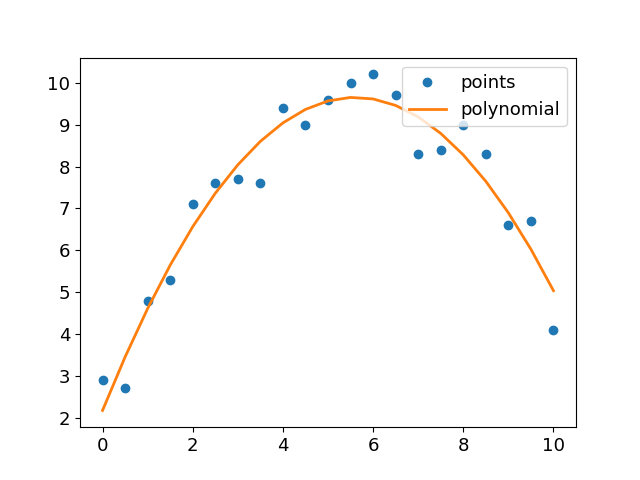
\includegraphics[height=5.1cm,width=6.8cm]{Figure_1.png}
\label{Fig1}
\end{figure}
可以看出函数的条件数十分稳定,但是算法A条件数的界当$x \rightarrow 0$时会很大,说明在计算机实际计算$f(x)$时,算法A在$x$很小时性质并不良好。
\end{proof}
\subsection*{Problem \uppercase\expandafter{\romannumeral10}}
\begin{proof}[\textbf{Solution.}]
根据范数的定义(此处理解略有歧义,因此给出两种可能情况的对应结果,具体请看下文中的补充部分)和\textbf{Definition 4.68}可得
\begin{equation}
   \mathrm{cond}_f(a_0,a_1,\dots,a_{n-1}) = \frac{1}{|r|}\sum^{n-1}_{i=0}\left|a_i\frac{\partial r}{\partial a_i}\right|.
\end{equation}
由于$F(a_0,a_1,\dots,a_{n-1},r) = a_0 + a_1r+\dots+a_{n-1}r^{n-1} + r^n = 0$,因此由隐函数求导有
\begin{equation}
   \frac{\partial r}{\partial a_i} = -\frac{F_{a_i}}{F_r} = \frac{-r^{i}}{a_1+a_2r + \dots + (n-1)a_{n-1}r^{n-2} + nr^{n-1}},
\end{equation}
从而
\begin{equation}
   \mathrm{cond}_f(a_0,a_1,\dots,a_{n-1}) = \frac{\sum^{n-1}_{i=0}\left|a_ir^i\right|}{|a_1r+a_2r^2+\dots+(n-1)a_{n-1}r^{n-1}+nr^{n}|}.
\end{equation}
进一步,对于Wilkinson一例,有$n=r=p > 0$,
\begin{equation}
   \mathrm{cond}_f(a_0,a_1,\dots,a_{p-1}) = \frac{-p^p+\prod^{p}_{k=1}(p+k)}{p\sum^{p}_{i=1}\prod^{p}_{k = 1,k\neq i}(p-k)} = \frac{-p^p+\prod^{p}_{k=1}(p+k)}{p!}.
\end{equation}
由于
\begin{equation}
   \frac{\prod^{p}_{k=1}(p+k)}{p^p} = (1+\frac{1}{p})(1+\frac{2}{p})\dots(1+1) > 2,
\end{equation}
因此有
\begin{equation}
   \mathrm{cond}_f(a_0,a_1,\dots,a_{p-1}) \geq \frac{p^p}{p!}.
\end{equation}
这与\textbf{Example 4.64}的结果十分类似,它们都可以说明当$p$足够大时,$f$的小扰动会造成根的巨大改变。

\textbf{补充}:如果严格按照课本(4.38)构造$1 \times n$矩阵的范数,那么此时的1范数并非向量的1范数,而应该指的是行向量矩阵的1范数,即
\begin{equation}
   \mathrm{cond}_f(a_0,a_1,\dots,a_{n-1}) = \frac{1}{|r|}\max_{i=0,1,\dots,n-1}\left|a_i\frac{\partial r}{\partial a_i}\right|=\frac{\max_{i=0,1,\dots,n-1}\left|a_ir^i\right|}{|a_1r+a_2r^2+\dots+(n-1)a_{n-1}r^{n-1}+nr^{n}|}.
\end{equation}
对于Wilkinson一例,类似上文分析则对应有$n=r=p > 0$,
\begin{equation}
   \mathrm{cond}_f(a_0,a_1,\dots,a_{p-1}) = \frac{\max_{i=0,1,\dots,p-1}\left|a_ip^i\right|}{p!}\geq\frac{p^{p-1}}{p!}.
\end{equation}
这样也可以得到类似的结果和分析。由于此处矩阵的维数$1 \times n$的特殊性,此处的范数可以有两种理解,\textbf{但是思路都是类似的}。都给出对应的结果,特此补充。
\end{proof}
\subsection*{Problem \uppercase\expandafter{\romannumeral11}}
\begin{proof}[\textbf{Solution.}]
仿照\textbf{Example 4.29},在规范化FPN $(\beta,p,L,U)$中取$\beta = 2, p = 2, L=-1,U = 1$。此时根据\textbf{Definition 4.38}计算$a = (2)_{10} = (1.0)_2 \times 2^1$与$a = (3)_{10} = (1.1)_2 \times 2^1$的商。

由于$\frac{2}{3}= (0.1010\dots)_2$,\textbf{Definition 4.38}第2步后(寄存器精度为4)$\frac{a}{b} = (0.101)_2 \times 2^0$,第3步后$\frac{a}{b} = (1.01)_2 \times 2^{-1}$,第5步后(round to even)$\frac{a}{b} = (1.0)_2 \times 2^{-1}$,从而有
\begin{equation}
    \mathrm{fl}(\frac{2}{3}) = (1.0)_2 \times 2^{-1},
\end{equation}
进而
\begin{equation}
    -\delta = \frac{\frac{2}{3}-\mathrm{fl}(\frac{2}{3})}{\frac{2}{3}} = \frac{(0.0101\dots)_2 \times 2^{-1}}{(1.0101\dots)_2 \times 2^{-1}} = \frac{1}{4}.
\end{equation}
然而$|\delta| = \frac{1}{4} = \epsilon_u$,与\textbf{Lemma 4.39}矛盾!
\end{proof}
\subsection*{Problem \uppercase\expandafter{\romannumeral12}}
\begin{proof}[\textbf{Solution.}]
在IEEE 754标准下,由于根在区间$[128,129]$之间,因此此时若将FPN表示成(4.1)的形式,有$e = 7$,因此此时FPN系统中相邻两个浮点数间距为
\begin{equation}
    \Delta = \epsilon_M \times 2^{e} = 2^{-16} > 10^{-6}.
\end{equation}
因此绝对精度并不能保证达到$10^{-6}$以内。
\end{proof}
\subsection*{Problem \uppercase\expandafter{\romannumeral13}}
\begin{proof}[\textbf{Solution.}]
求解三次样条的插值问题(不失一般性,以complete cubic spline为例,其他边界条件类似),根据\textbf{Theorem 3.7},可以发现先需求解课本式(3.15)给出的线性方程组得到各$m_i\;(i=1,2,\dots,N)$,再根据$m_i$的值带入课本\textbf{Lemma 3.3}式(3.6)的方程组得到多项式的各个系数。因此,若其中两个插值点$x_i,x_{i+1}$的距离远小于其余相邻插值点的间距,产生的误差可能会来自式(3.15)和(3.6)两步。

首先是求解(3.15)的线性方程组。$x_i,x_{i+1}$间距很小意味着相对来说$\lambda_i$和$\mu_{i+1}$会十分趋近0,而$\lambda_{i+1}$和$\mu_{i}$会十分趋近与1。按照题目给出的提示,此时(3.15)的矩阵的条件数(由于范数的等价性,不妨本题的条件数均以2范数为基准)似乎应该很大。然而,根据我在python的计算,结果并非如此。

不失一般性,我构造了等间距1的一系列插值点,并使最中间的两个插值点间距为0.01。改变插值点个数从6-102个,对应的矩阵(维度从4-100)的条件数存入了\verb|condition_number.txt|中并作图如下。
\begin{figure}[H]
\centering
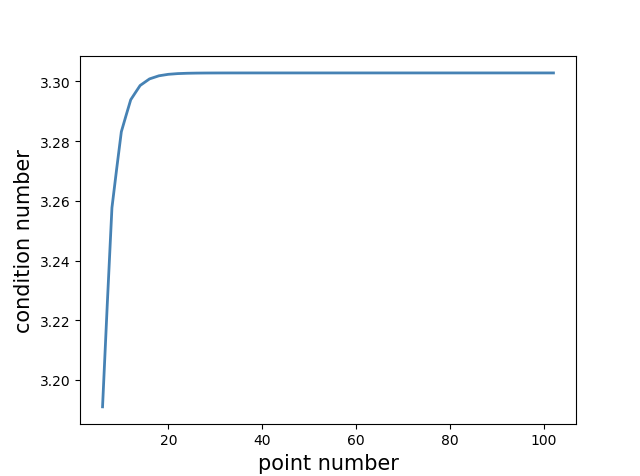
\includegraphics[height=5.1cm,width=6.8cm]{Figure_6.png}
\label{Fig1}
\end{figure}
可以发现,随着插值点个数增多,矩阵条件数略有增大,并且最终稳定在$3.30283$左右,并没有出现异常。因此可以认为(3.15)能够求解得到较为稳定的$m_i\;(i=1,2,\dots,N)$。

由此考虑第二步:求解(3.6)。由于$c_{i,0}=f_i$,$c_{i,1}=m_i$,在求解$c_{i,0},c_{i,1}$的过程中并不会出现异常情况。然而,若$x_i,x_{i+1}$的距离非常近,则由样条函数连续可微知此时$m_i \sim m_{i+1}$(即$\frac{m_{i+1}}{m_i} \rightarrow 1$,下同);并且,由样条函数在$x_i$处的Taylor展开以及差商的连续性可知此时还有$K_i = f[x_i,x_{i+1}] \sim m_i$。也就是说,$m_i,m_{i+1},K_i$三者此时近似相等。

由此,在计算$c_{i,2}=\frac{3K_i-2m_i-m_{i+1}}{x_{i+1}-x_i}$和$c_{i,3}=\frac{m_i+m_{i+1}-2K_i}{(x_{i+1}-x_i)^2}$时,二者的分子和分母都会十分接近0!从而导致在计算$c_{i,2}$和$c_{i,3}$分子分母时,会出现\textbf{Example 4.48}所示的巨量消失现象,导致结果不准确。

综上所述,结果的不准确出现在了求解课本式(3.6)一步中分子分母的加减法运算产生的巨量消失。
\end{proof}

\section*{Programming assignments}
本次编程作业使用C++和python共同编写,python作画图用。其中C++部分采用Makefile文件对编译进行统一管理。具体地,在Makefile所在目录下输入\verb|make|
即可完成编译,得到可执行文件\verb|test|。对其运行即可得到各小题的输出结果,具体内容将按问题顺序分别作出说明。
\subsection*{Problem A}
题目中给出的函数的三种不同表达形式在$[0.99,1.01]$等间距插值结果在\verb|point_value.txt|中给出了完整的展示和说明。限于篇幅,请自行查阅该文本文件,此处不再列出具体的值。

进一步,三个函数在$[0.996,1.004]$计算得到的函数值的各自放大图像及对比图如下图所示。
\begin{figure}[H]
\centering
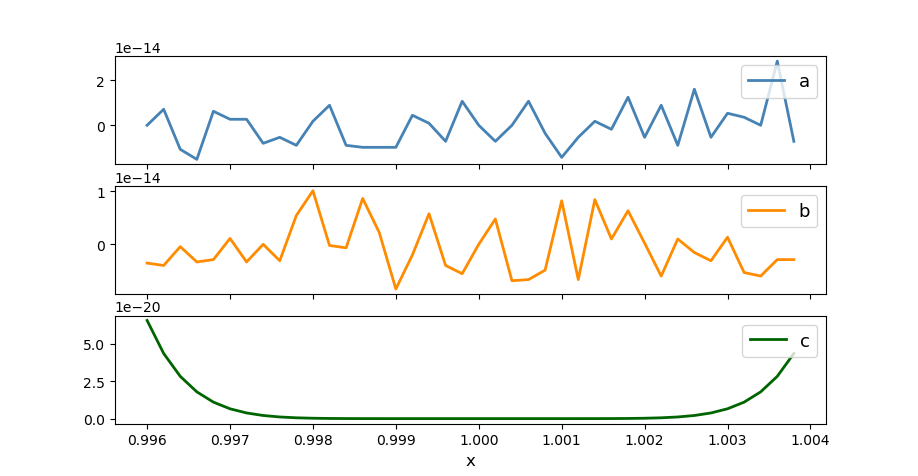
\includegraphics[height=5.4cm,width=10.7cm]{Figure_2.png}
\label{Fig1}
\end{figure}
\begin{figure}[H]
\centering
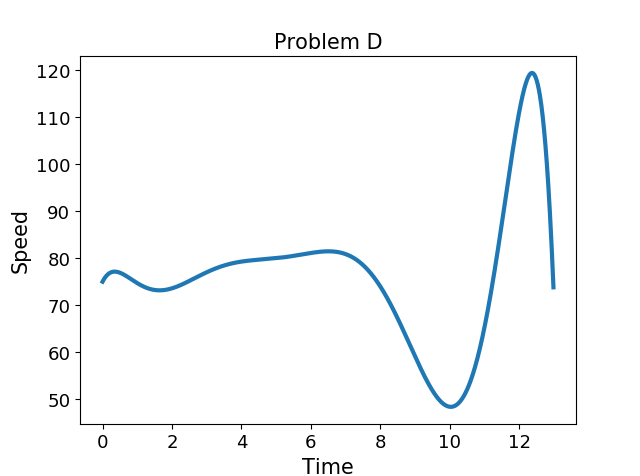
\includegraphics[height=5.4cm,width=11cm]{Figure_3.png}
\label{Fig1}
\end{figure}
理论上说,三个函数在$x$接近1时都应该趋向0。但是从图像中可以很明显地看出三个函数表达形式的误差并不相同。对比(4.49 a)和(4.49 b),可以发现(4.49 b)形式的误差总体小于(4.49 a)的误差,这是因为(4.49 b)的二元运算次数为15次,远远小于(4.49 a)中的43次,从而避免了大量的舍入误差。另一方面,对比图中,似乎(4.49 c)都是0,发生了巨量消失。然而通过单独绘图以及\verb|point_value.txt|中的数据,可以看出并没有明显发生这种情况。此外,只有(4.49 c)的值是连续的。因此综合考虑,(4.49 a)的形式误差最大,其次是(4.49 b),误差最小的是(4.49 c)。
\subsection*{Problem B}
首先,根据\textbf{Definition 4.17},程序相应输出
\begin{shaded}
\begin{verbatim}
UFL = 0.5
OFL = 3.5
\end{verbatim}
\end{shaded}
其次,对于FPN系统的全体浮点数,程序相应输出
\begin{shaded}
\begin{verbatim}
All numbers in F are: 
0.5, -0.5, 0.625, -0.625, 0.75, -0.75, 0.875, -0.875, 1, -1, 1.25, -1.25, 1.5, -1.5,
1.75, -1.75, 2, -2, 2.5, -2.5, 3, -3, 3.5, -3.5, 0. 
25 numbers in total.
\end{verbatim}
\end{shaded}
而25个FPN也印证了\textbf{Corollary 4.19}:$\quad \#F = 2^P(U-L+1)+1 = 8(1+1+1)+1=25$。进一步的,FPN系统的全体浮点数在实轴上表示如下图所示。
\begin{figure}[H]
\centering
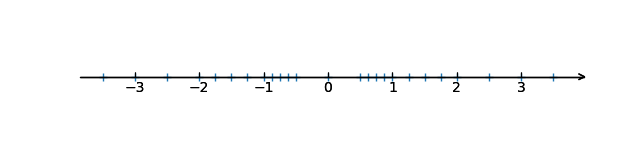
\includegraphics[height=2.8cm,width=11cm]{Figure_4.png}
\label{Fig1}
\end{figure}
此外,该FPN系统的非规格化浮点数由程序输出如下:
\begin{shaded}
\begin{verbatim}
All subnumbers are: 
0.125, -0.125, 0.25, -0.25, 0.375, -0.375. 
6 numbers in total.
\end{verbatim}
\end{shaded}
加上这些非规格化浮点数后的全体FPN在实轴上表示如下图所示。
\begin{figure}[H]
\centering
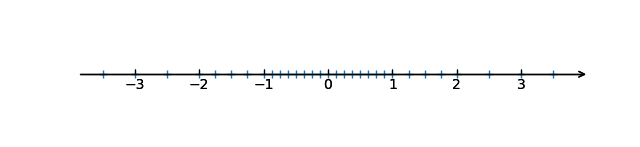
\includegraphics[height=2.8cm,width=11.2cm]{Figure_5.png}
\label{Fig1}
\end{figure}
\end{sloppypar}
\end{document}
